\documentclass[border=10pt]{standalone}
\usepackage{tikz}\usepackage{amsmath}\usetikzlibrary{arrows.meta,decorations.pathmorphing}
\begin{document}
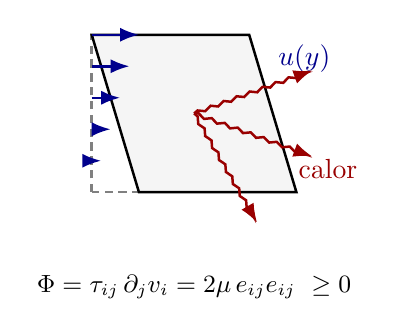
\begin{tikzpicture}[line width=0.9pt,>={Latex[length=2.4mm]}]
  % perfil de cizalla
  \draw[gray,densely dashed] (0,0) rectangle (2,2);
  \draw[fill=black!4] (0.6,0) -- (2.6,0) -- (2.0,2) -- (0,2) -- cycle;
  \foreach \y in {0.4,0.8,1.2,1.6,2.0} \draw[->,blue!55!black] (0,\y)--++({0.3*\y},0);
  \node[blue!55!black] at (2.7,1.7){$u(y)$};
  % calor saliente (ondulado)
  \foreach \a in {300,340,20}
     \draw[->,red!60!black,decorate,decoration={snake,amplitude=0.6pt,segment length=5pt}] (1.3,1.0)--++(\a:1.6);
  \node[red!60!black] at (3.0,0.3){calor};
  \node[align=center] at (1.3,-1.2){\small $\Phi=\tau_{ij}\,\partial_j v_i=2\mu\,e_{ij}e_{ij}\ \ge 0$};
\end{tikzpicture}
\end{document}
